%package list
\documentclass{article}
\usepackage[top=3cm, bottom=3cm, outer=3cm, inner=3cm]{geometry}
\usepackage{multicol}
\usepackage{graphicx}
\usepackage{url}
%\usepackage{cite}
\usepackage{hyperref}
\usepackage{array}
%\usepackage{multicol}
\newcolumntype{x}[1]{>{\centering\arraybackslash\hspace{0pt}}p{#1}}
\usepackage{natbib}
\usepackage{pdfpages}
\usepackage{multirow}
\usepackage[normalem]{ulem}
\useunder{\uline}{\ul}{}
\usepackage{svg}
\usepackage{xcolor}
\usepackage{listings}
\lstdefinestyle{ascii-tree}{
    literate={├}{|}1 {─}{--}1 {└}{+}1 
  }
\lstset{basicstyle=\ttfamily,
  showstringspaces=false,
  commentstyle=\color{red},
  keywordstyle=\color{blue}
}
%\usepackage{booktabs}
\usepackage{caption}
\usepackage{subcaption}
\usepackage{float}
\usepackage{array}

\newcolumntype{M}[1]{>{\centering\arraybackslash}m{#1}}
\newcolumntype{N}{@{}m{0pt}@{}}


%%%%%%%%%%%%%%%%%%%%%%%%%%%%%%%%%%%%%%%%%%%%%%%%%%%%%%%%%%%%%%%%%%%%%%%%%%%%
%%%%%%%%%%%%%%%%%%%%%%%%%%%%%%%%%%%%%%%%%%%%%%%%%%%%%%%%%%%%%%%%%%%%%%%%%%%%
\newcommand{\itemEmail}{rvaldiviase@unsa.edu.pe}
\newcommand{\itemStudent}{Ryan Fabian Valdivia Segovia}
\newcommand{\itemCourse}{Fundamentos de la programación 2}
\newcommand{\itemCourseCode}{1701213}
\newcommand{\itemSemester}{II}
\newcommand{\itemUniversity}{Universidad Nacional de San Agustín de Arequipa}
\newcommand{\itemFaculty}{Facultad de Ingeniería de Producción y Servicios}
\newcommand{\itemDepartment}{Departamento Académico de Ingeniería de Sistemas e Informática}
\newcommand{\itemSchool}{Escuela Profesional de Ingeniería de Sistemas}
\newcommand{\itemAcademic}{2023 - B}
\newcommand{\itemInput}{Del 11 de Octubre 2023}
\newcommand{\itemOutput}{Al 16 de Octubre 2023}
\newcommand{\itemPracticeNumber}{06}
\newcommand{\itemTheme}{ArrayList}
%%%%%%%%%%%%%%%%%%%%%%%%%%%%%%%%%%%%%%%%%%%%%%%%%%%%%%%%%%%%%%%%%%%%%%%%%%%%
%%%%%%%%%%%%%%%%%%%%%%%%%%%%%%%%%%%%%%%%%%%%%%%%%%%%%%%%%%%%%%%%%%%%%%%%%%%%

\usepackage[english,spanish]{babel}
\usepackage[utf8]{inputenc}
\AtBeginDocument{\selectlanguage{spanish}}
\renewcommand{\figurename}{Figura}
\renewcommand{\refname}{Referencias}
\renewcommand{\tablename}{Tabla} %esto no funciona cuando se usa babel
\AtBeginDocument{%
	\renewcommand\tablename{Tabla}
}

\usepackage{fancyhdr}
\pagestyle{fancy}
\fancyhf{}
\setlength{\headheight}{30pt}
\renewcommand{\headrulewidth}{1pt}
\renewcommand{\footrulewidth}{1pt}
\fancyhead[L]{\raisebox{-0.2\height}{
\includegraphics[width=3cm]{img/logo_episunsa.png}}}
\fancyhead[C]{\fontsize{7}{7}\selectfont	\itemUniversity \\ \itemFaculty \\ \itemDepartment \\ \itemSchool \\ \textbf{\itemCourse}}
\fancyhead[R]{\raisebox{-0.2\height}{
\includegraphics[width=1.2cm]{img/logo_abet}}}
\fancyfoot[L]{Estudiante Ryan Valdivia}
\fancyfoot[C]{\itemCourse}
\fancyfoot[R]{Página \thepage}

% para el codigo fuente
\usepackage{listings}
\usepackage{color, colortbl}
\definecolor{dkgreen}{rgb}{0,0.6,0}
\definecolor{gray}{rgb}{0.5,0.5,0.5}
\definecolor{mauve}{rgb}{0.58,0,0.82}
\definecolor{codebackground}{rgb}{0.95, 0.95, 0.92}
\definecolor{tablebackground}{rgb}{0.8, 0, 0}

\lstset{frame=tb,
	language=bash,
	aboveskip=3mm,
	belowskip=3mm,
	showstringspaces=false,
	columns=flexible,
	basicstyle={\small\ttfamily},
	numbers=none,
	numberstyle=\tiny\color{gray},
	keywordstyle=\color{blue},
	commentstyle=\color{dkgreen},
	stringstyle=\color{mauve},
	breaklines=true,
	breakatwhitespace=true,
	tabsize=3,
	backgroundcolor= \color{codebackground},
}

\begin{document}
	
	\vspace*{10px}
	
	\begin{center}	
		\fontsize{17}{17} \textbf{ Informe de Laboratorio \itemPracticeNumber}
	\end{center}
	\centerline{\textbf{\Large Tema: \itemTheme}}
	%\vspace*{0.5cm}	

	\begin{flushright}
		\begin{tabular}{|M{2.5cm}|N|}
			\hline 
			\rowcolor{tablebackground}
			\color{white} \textbf{Nota}  \\
			\hline 
			     \\[30pt]
			\hline 			
		\end{tabular}
	\end{flushright}	

	\begin{table}[H]
		\begin{tabular}{|x{4.7cm}|x{4.8cm}|x{4.8cm}|}
			\hline 
			\rowcolor{tablebackground}
			\color{white} \textbf{Estudiante} & \color{white}\textbf{Escuela}  & \color{white}\textbf{Asignatura}   \\
			\hline 
			{\itemStudent \par \itemEmail} & \itemSchool & {\itemCourse \par Semestre: \itemSemester \par Código: \itemCourseCode}     \\
			\hline 			
		\end{tabular}
	\end{table}		
	
	\begin{table}[H]
		\begin{tabular}{|x{4.7cm}|x{4.8cm}|x{4.8cm}|}
			\hline 
			\rowcolor{tablebackground}
			\color{white}\textbf{Laboratorio} & \color{white}\textbf{Tema}  & \color{white}\textbf{Duración}   \\
			\hline 
			\itemPracticeNumber & \itemTheme & 04 horas   \\
			\hline 
		\end{tabular}
	\end{table}
	
	\begin{table}[H]
		\begin{tabular}{|x{4.7cm}|x{4.8cm}|x{4.8cm}|}
			\hline 
			\rowcolor{tablebackground}
			\color{white}\textbf{Semestre académico} & \color{white}\textbf{Fecha de inicio}  & \color{white}\textbf{Fecha de entrega}   \\
			\hline 
			\itemAcademic & \itemInput &  \itemOutput  \\
			\hline 
		\end{tabular}
	\end{table}
	
	\section{Tarea}
	\begin{itemize}
		\subsection{Videojuego}
			\item Cree un Proyecto llamado Laboratorio6.
			\item Usted deberá crear las dos clases Soldado.java y VideoJuego3.java. Puede reutilizar lo desarrollado en Laboratorios anteriores.
			\item Del Soldado nos importa el nombre, puntos de vida, fila y columna (posición en el tablero).
			\item El juego se desarrollará en el mismo tablero de los laboratorios anteriores. Pero ahora el
tablero debe ser un ArrayList bidimensional.
			\item Tendrá 2 Ejércitos. Inicializar el tablero con n soldados aleatorios entre 1 y 10 para cada
Ejército. Cada soldado tendrá un nombre autogenerado: Soldado0X1, Soldado1X1, etc., un
valor de puntos de vida autogenerado aleatoriamente [1..5], la fila y columna también
autogenerados aleatoriamente (no puede haber 2 soldados en el mismo cuadrado). Se debe
mostrar el tablero con todos los soldados creados (distinguir los de un ejército de los del otro
ejército). Además de los datos del Soldado con mayor vida de cada ejército, el promedio de
puntos de vida de todos los soldados creados por ejército, los datos de todos los soldados por
ejército en el orden que fueron creados y un ranking de poder de todos los soldados creados
por ejército (del que tiene más nivel de vida al que tiene menos) usando 2 diferentes algoritmos de ordenamiento. Finalmente, que muestre qué ejército ganará la batalla (indicar
la métrica usada para decidir al ganador de la batalla).
	\end{itemize}
		
	\section{Equipos, materiales y temas utilizados}
	\begin{itemize}
		\item Sistema Operativo Windows 11 Home Single Language 64 bits 22621.2283
		\item VIM 9.0.
		\item Visual Studio Code 64 bits 1.82.2
		\item OpenJDK 64-Bits 11.0.16.1
		\item Git 2.41.0.windows.1
		\item Cuenta en GitHub con el correo institucional. 
	\end{itemize}
	
	\section{URL de Repositorio Github}
	\begin{itemize}
		\item URL del Repositorio GitHub para clonar o recuperar.
		\item \url{https://github.com/RyanValdivia/fp2-23b.git}
		\item URL para el laboratorio 06 en el Repositorio GitHub.
		\item \url{https://github.com/RyanValdivia/fp2-23b/tree/main/fase02/lab06}
	\end{itemize}
	
	\section{Actividades}
	\subsection{Actividad 1}
	
	\begin{itemize}	
		\item En primer lugar, realicé un commit conteniendo el código de la clase Soldado.java, requerido para la clase principal
	\end{itemize}	
	\begin{lstlisting}[language=bash,caption={Obteniendo la clase Soldado}][H]
		$ git log lab06
		commit b13def7c362a6359bf680d2606fd7da6dfe93911
		Author: RYAN VALDIVIA <rvaldiviase@unsa.edu.pe>
		Date:   Mon Oct 16 09:29:53 2023 -0500
			Anadiendo la clase Soldado para poder crear la lista bidimensional
	\end{lstlisting}
	\begin{itemize}	
		\item Conteniendo el siguiente código
	\end{itemize}
	\begin{lstlisting}[language=java,caption={Clase Soldado}, numbers=left][H]
public class Soldado {
    private String nombre;
    private int vida;
    private int fila;
    private int columna;

    public void setNombre(String s) {
        this.nombre = s;
    }

    public void setVida(int n) {
        this.vida = n;
    }

    public void setFila(int n) {
        this.fila = n;
    }

    public void setColumna(int n) {
        this.columna = n;
    }

    public String getNombre() {
        return nombre;
    }

    public int getVida() {
        return vida;
    }

    public int getFila() {
        return fila;
    }

    public int getColumna() {
        return columna;
    }
}
	\end{lstlisting}
	\begin{itemize}	
		\item Para este problema, reutilicé diferentes cosas que hice en el laboratorio anterior, como el sistema para crear las coordenadas de los soldados, usando arreglos de números aleatorios.
	\end{itemize}
	\begin{lstlisting}[language=java,caption={Números aleatorios}, numbers=left][H]
	public static int[] numerosRandom(int q) {
        int[] nums = new int[q];
        for (int i = 0; i < nums.length; i++) {
            nums[i] = nums.length;
        }
        for (int i = 0; i < q; i++) {
            int n;
            do {
                n = (int) (Math.random() * 10);
            } while (estaEnArreglo(nums, n, i));
            nums[i] = n;
        }
        return nums;
    }
    public static boolean estaEnArreglo(int[] arreglo, int num, int indice) {
        for (int i = 0; i < indice; i++) {
            if (arreglo[i] == num) {
                return true;
            }
        }
        return false;
    }
	\end{lstlisting}
	\begin{itemize}	
		\item Solo que, en este caso, son dos ejércitos y dos soldados de ambos ejércitos no pueden estar en la misma casilla, asi que adapté este código para que no se generen dos pares ordenados iguales.
	\end{itemize}
	\begin{lstlisting}[language=java,caption={Método main}, numbers=left][H]
		Scanner sc = new Scanner(System.in);
        ArrayList<ArrayList<Soldado>> tablero = new ArrayList<>(10);
        int ej1 = (int) ((Math.random() * 10) + 1);
        int ej2 = (int) ((Math.random() * 10) + 1);
        int[] filas1 = numerosRandom(ej1);
        int[] columnas1 = numerosRandom(ej1);
        int[] filas2;
        int[] columnas2;
        do {
            filas2 = numerosRandom(ej2);
            columnas2 = numerosRandom(ej2);
        } while (!diffCoordenadas(filas1, filas2, columnas1, columnas2));
	\end{lstlisting}
	\begin{itemize}	
		\item Aqui primero inicialicé los objetos necesarios, como el Scanner (que usaré después) y la Lista Bidimensional, además de conseguir los arreglos que formaran las coordenadas de los objetos de ambos ejércitos, asegurándome, con esa estructura do-while, que dos pares ordenados de ambos ejércitos jamás sean iguales, para que dos soldados nunca estén en una misma casilla, usando otro método.
	\end{itemize}
	\begin{lstlisting}[language=java,caption={Coordenadas diferentes}, numbers=left][H]
	public static boolean diffCoordenadas(int[] filas1, int[] filas2, int[] columnas1, int[] columnas2) {
        if (filas1.length > filas2.length) {
            for (int i = 0; i < filas2.length; i++) {
                if (filas1[i] == filas2[i] && columnas1[i] == columnas2[i]) {
                    return false;
                }
            }
        } else {
            for (int i = 0; i < filas1.length; i++) {
                if (filas1[i] == filas2[i] && columnas1[i] == columnas2[i]) {
                    return false;
                }
            }
        }
        return true;
    }
	\end{lstlisting}	
	\begin{itemize}	
		\item Este método comprueba que, dados dos arreglos de coordenadas, no hayan pares ordenados iguales.
		\item Lo siguiente era inicializar el arreglo para empezar a añadir los soldados, ya que ya tenemos sus localizaciones. Para esto, creé un método específico para inicializar el ArrayList.
	\end{itemize}
	\begin{lstlisting}[language=java,caption={Inicializar la lista}, numbers=left][H]
	 public static void inicializarLista(ArrayList<ArrayList<Soldado>> army) {
        for (int i = 0; i < 10; i++) {
            army.add(new ArrayList<>());
        }
        for (int i = 0; i < 10; i++) {
            for (int j = 0; j < 10; j++) {
                army.get(i).add(new Soldado());
                army.get(i).get(j).setNombre("          ");
            }
        }

    }
	\end{lstlisting}
	\begin{itemize}	
		\item Este método inicia instanciando las Listas (Para utilizar una lista bidimensional) y posteriormente, instancia los objetos en cada lista con el atributo de nombre como un String vacío, esto es para comodidad al momento de imprimir todo el tablero.
		\item Una vez ya inicializado e instanciado, toca añadir a todos los soldados, dados las coordenadas ya generadas de forma aleatoria, para esto, creé otro método.
	\end{itemize}
	\begin{lstlisting}[language=java,caption={Desplegando nuestras tropas}, numbers=left][H]
	 public static void desplegarEjercito(ArrayList<ArrayList<Soldado>> army, int[] filas, int[] columnas, int ej) {
        for (int i = 0; i < filas.length; i++) {
            int v = (int) ((Math.random() * 5) + 1);
            army.get(filas[i]).get(columnas[i]).setNombre("Soldado" + i + "X" + ej);
            army.get(filas[i]).get(columnas[i]).setVida(v);
            army.get(filas[i]).get(columnas[i]).setFila(filas[i]);
            army.get(filas[i]).get(columnas[i]).setColumna(columnas[i]);
        }
    }
	\end{lstlisting}
	\begin{itemize}	
		\item Una vez ya desplegados los dos ejércitos, viene la parte algo complicada, mostrar el tablero, para lo cual reciclaré el código del anterior laboratorio, modificandolo para que funcione con las nuevas medidas.
		\item Comenzaré con el método para mostrar el tablero, imprimiendo los atributos 'Nombre' de todos los objetos de la lista (Por eso fue que inicialicé todos los objetos con un String vacío por defecto).
	\end{itemize}
	\begin{lstlisting}[language=java,caption={Mostrar el tablero}, numbers=left][H]
	 public static void mostrarTablero(ArrayList<ArrayList<Soldado>> army) {
        System.out.println(crearTecho());
        for (int i = 0; i < 10; i++) {
            System.out.println(separadorSup());
            for (int j = 0; j < 10; j++) {
                if (j == 10 - 1) {
                    System.out.print("| " + army.get(i).get(j).getNombre() + " |");
                } else {
                    System.out.print("| " + army.get(i).get(j).getNombre() + " ");
                }
            }
            System.out.println();
            System.out.println(separadorInf());
        }
    }
    public static String crearTecho() {
        String franky = "";
        for (int i = 0; i < 131; i++) {
            franky += "_";
        }
        return franky;
    }

    public static String separadorInf() {
        String franky = "";
        for (int i = 0; i < 131; i++) {
            if (i % 13 == 0) {
                System.out.print("|");
            } else {
                System.out.print("_");
            }
        }
        return franky;
    }

    public static String separadorSup() {
        String franky = "";
        for (int i = 0; i < 131; i++) {
            if (i % 13 == 0) {
                System.out.print("|");
            } else {
                System.out.print(" ");
            }
        }
        return franky;
    }
	\end{lstlisting}
	
	\begin{itemize}
		\item Imprimiendo esto al momento de ejecutar el código.
	\end{itemize}
	
	\begin{figure}[H]
		\centering
	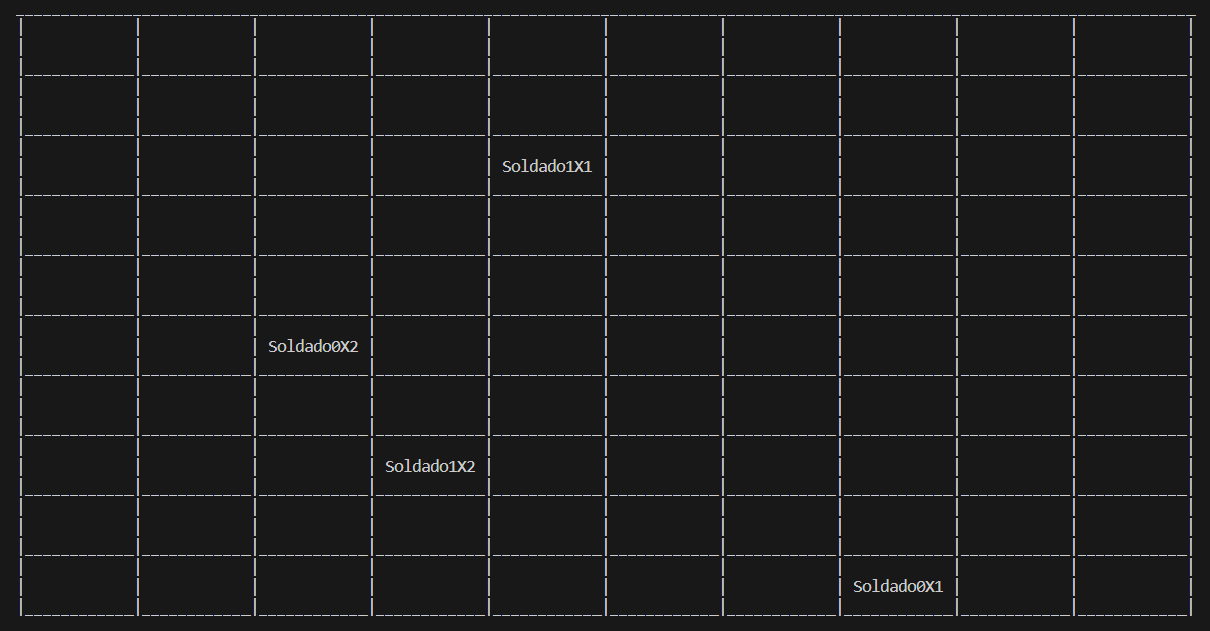
\includegraphics[width=0.8\textwidth,keepaspectratio]{img/captura1.png}
		%\includesvg{img/automata.svg}
		%\label{img:mot2}
		%\caption{Product backlog.}
	\end{figure}
	
	\begin{itemize}	
		\item Una vez terminado el tablero, pasé a trabajar el resto de requerimientos para el programa.
		\item Ahora debía mostrar el soldado con mayor nivel de vida, para esto, decidí crear un arreglo simple a partir de la lista bidimensional que ya tenía, para que sea mucho más sencillo de trabajar luego.
	\end{itemize}
	\begin{lstlisting}[language=java,caption={De Lista a Arreglo}, numbers=left][H]
	  public static ArrayList<Soldado> crearLista(ArrayList<ArrayList<Soldado>> army, int[] filas, int[] columnas) {
        ArrayList<Soldado> nuevo = new ArrayList<>();
        for (int i = 0; i < filas.length; i++) {
            nuevo.add(army.get(filas[i]).get(columnas[i]));
        }
        return nuevo;
    }
	 public static Soldado[] convertirArray(ArrayList<Soldado> army) {
        Soldado[] nuevo = new Soldado[army.size()];
        for (int i = 0; i < nuevo.length; i++) {
            nuevo[i] = army.get(i);
        }
        return nuevo;
    }
	\end{lstlisting}
	\begin{itemize}	
		\item Con estos métodos, convierto mi lista bidimensional en una lista normal, y luego en un arreglo simple.
		\item Además, reusé el método para mostrar un soldado y mostrar el ejército a partir de un arreglo.
	\end{itemize}
	\begin{lstlisting}[language=java,caption={Mostrar soldado y ejército}, numbers=left][H]
	  public static void mostrarSoldado(Soldado[] army, int i) {
        String columna;
        System.out.println("Nombre: " + army[i].getNombre());
        System.out.println("Vida: " + army[i].getVida() + " HP");
        switch (army[i].getColumna() + 1) {
            case 1:
                columna = "A";
                break;
            case 2:
                columna = "B";
                break;
            case 3:
                columna = "C";
                break;
            case 4:
                columna = "D";
                break;
            case 5:
                columna = "E";
                break;
            case 6:
                columna = "F";
                break;
            case 7:
                columna = "G";
                break;
            case 8:
                columna = "H";
                break;
            case 9:
                columna = "I";
                break;
            case 10:
                columna = "J";
                break;
            default:
                columna = "K";
                break;
        }
        System.out.println("Posicion: " + (army[i].getFila() + 1) + "-" + columna);
    }
    
    public static void mostrarEjercito(Soldado[] army, int ej) {
        System.out.println("Ejercito " + ej);
        for (int i = 0; i < army.length; i++) {
            mostrarSoldado(army, i);
        }
        System.out.println();
    }
	\end{lstlisting}
	
	\begin{itemize}	
		\item Ahora si, muestro el soldado con mayor nivel de vida de cada ejército, además del nivel total y promedio de vida de cada ejército.
	\end{itemize}
	\begin{lstlisting}[language=java,caption={Mayor nivel de vida}, numbers=left][H]
	 public static void soldadoMayorVida(Soldado[] army, int ej) {
        int max = 0;
        for (int i = 0; i < army.length; i++) {
            if (army[i].getVida() > army[max].getVida()) {
                max = i;
            }
        }
        System.out.println("El soldado con mayor vida del ejercito " + ej + " es: ");
        mostrarSoldado(army, max);
        System.out.println();
    }
     public static void mostrarTotalYPromedio(Soldado[] army, int ej) {
        int total = 0;
        for (int i = 0; i < army.length; i++) {
            total += army[i].getVida();
        }
        System.out.println("El nivel de vida total del ejercito " + ej + " es: " + total);
        System.out.println("El nivel de vida promedio del ejercito " + ej + " es: " + total * 1.0 / army.length);
        System.out.println();
    }
	\end{lstlisting}
	\begin{itemize}	
		\item Mostrando lo siguiente al momento de ejecutar el código (Siguiendo con la anterior captura).
	\end{itemize}
	
	\begin{figure}[H]
		\centering
	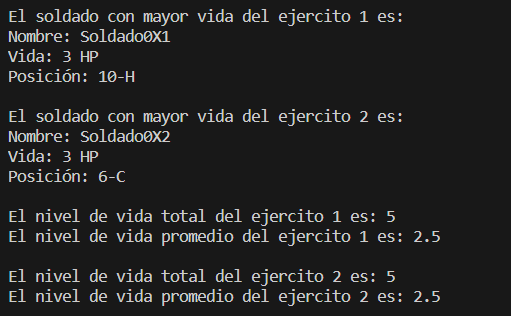
\includegraphics[width=0.8\textwidth,keepaspectratio]{img/captura2.png}
		%\includesvg{img/automata.svg}
		%\label{img:mot2}
		%\caption{Product backlog.}
	\end{figure}
	\begin{itemize}	
		\item También realicé el método para mostrar todo el ejército según el orden de creación de los objetos.
	\end{itemize}
	
	\begin{lstlisting}[language=java,caption={Mostrando el ejército}, numbers=left][H]
	 public static void mostrarEjercito(Soldado[] army, int ej) {
        System.out.println("Ejercito " + ej);
        for (int i = 0; i < army.length; i++) {
            mostrarSoldado(army, i);
        }
        System.out.println();
    }
	\end{lstlisting}
	\begin{itemize}	
		\item Mostrando lo siguiente al momento de ejecutar.
	\end{itemize}
	
	\begin{figure}[H]
		\centering
	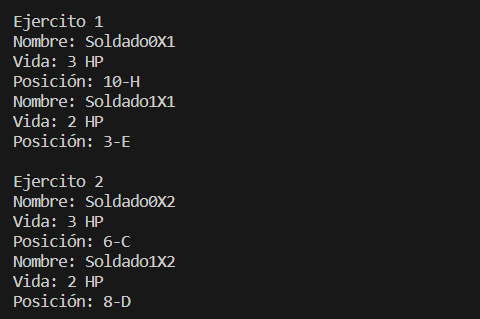
\includegraphics[width=0.8\textwidth,keepaspectratio]{img/captura3.png}
		%\includesvg{img/automata.svg}
		%\label{img:mot2}
		%\caption{Product backlog.}
	\end{figure}
	
	\begin{itemize}	
		\item A continuación falta lo último, que es ordenar los soldados, mostrarlos ya ordenados y determinar cuál ejército gana.
		\item Entonces, reciclé los algoritmos de ordenamiento del laboratorio anterior.
	\end{itemize}
	
	\begin{lstlisting}[language=java,caption={Algoritmos de ordenamiento}, numbers=left][H]
	 public static void ordenamientoInsercion(Soldado[] army) {
        for (int i = 1; i < army.length; i++) {
            Soldado valor = army[i];
            int j = i;
            for (j = i; 0 < j && army[j - 1].getVida() < valor.getVida(); j--) {
                army[j] = army[j - 1];
            }
            army[j] = valor;
        }
    }

    public static void ordenamientoBurbuja(Soldado[] army) {
        for (int i = 0; i < army.length; i++) {
            for (int j = 0; j < army.length - 1; j++) {
                if (army[j].getVida() < army[j + 1].getVida()) {
                    intercambiar(army, j, j + 1);
                }
            }
        }
    }

    public static void intercambiar(Soldado[] flota, int i, int j) {
        Soldado temp;
        temp = flota[i];
        flota[i] = flota[j];
        flota[j] = temp;
    }
	\end{lstlisting}
	\begin{itemize}	
		\item Para esto, una vez ya implementado, hicé un menú para el usuario como en el anterior trabajo, en el método main, además de armar todos los métodos realizados.
	\end{itemize}
	\begin{lstlisting}[language=java,caption={Método main}, numbers=left][H]
	 	Soldado[] ejercito1 = convertirArray(crearLista(tablero, filas1, columnas1));
        Soldado[] ejercito2 = convertirArray(crearLista(tablero, filas2, columnas2));
        System.out.println();
        soldadoMayorVida(ejercito1, 1);
        soldadoMayorVida(ejercito2, 2);
        mostrarTotalYPromedio(ejercito1, 1);
        mostrarTotalYPromedio(ejercito2, 2);
        mostrarEjercito(ejercito1, 1);
        mostrarEjercito(ejercito2, 2);

        System.out.println("Bajo que criterio le gustaria ordenar los ejercitos?");
        System.out.println("1. Burbuja");
        System.out.println("2. Insercion");
        switch (sc.nextInt()) {
            case 1:
                ordenamientoBurbuja(ejercito1);
                ordenamientoBurbuja(ejercito2);
                break;
            case 2:
                ordenamientoInsercion(ejercito1);
                ordenamientoBurbuja(ejercito2);
                break;
            default:
        }
        System.out.println("Ranking segun vida (Del mayor al menor): ");
        mostrarEjercito(ejercito1, 1);
        mostrarEjercito(ejercito2, 2);
	\end{lstlisting}
	
	\begin{itemize}	
		\item Para probar esta parte, hice otra ejecución del programa, ya que los ejércitos ya estaban ordenados.
		\item Siendo el ejército ordenado por orden de creación el siguiente:
	\end{itemize}
	
	\begin{figure}[H]
		\centering
	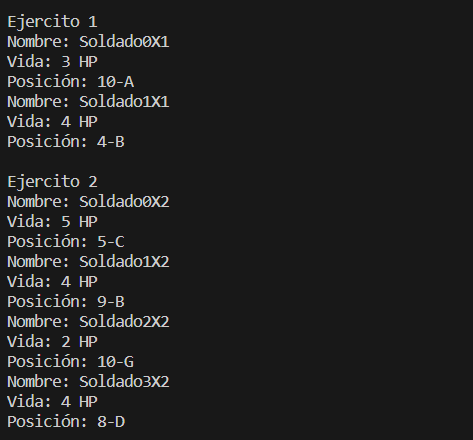
\includegraphics[width=0.6\textwidth,keepaspectratio]{img/captura4.png}
		%\includesvg{img/automata.svg}
		%\label{img:mot2}
		%\caption{Product backlog.}
	\end{figure}
	
	\begin{itemize}	
		\item Quedando así una vez ya ordenados:
		
	\end{itemize}
	
	\begin{figure}[H]
		\centering
	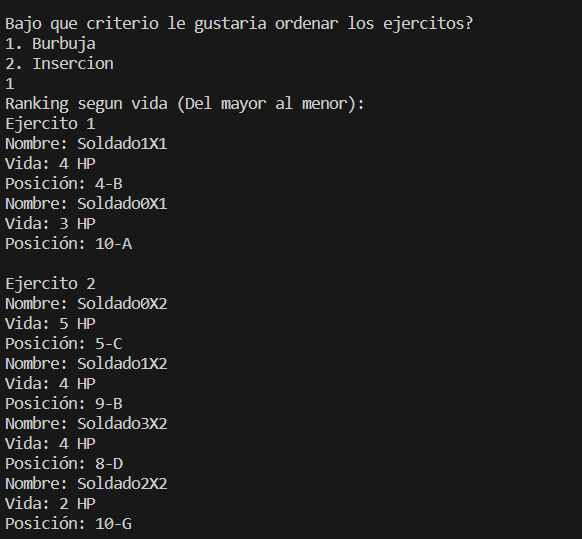
\includegraphics[width=0.6\textwidth,keepaspectratio]{img/captura5.png}
		%\includesvg{img/automata.svg}
		%\label{img:mot2}
		%\caption{Product backlog.}
	\end{figure}
	
	\begin{itemize}	
		\item Ya para terminar, solo faltaría saber qué ejército ganó, para esto, usé el criterio de qué ejército tiene más nivel de vida total.
	\end{itemize}
	
	\begin{lstlisting}[language=java,caption={Determinando el ganador}, numbers=left][H]
	 public static void ejercitoGanador(Soldado[] army1, Soldado[] army2) {
        int total1 = 0;
        int total2 = 0;
        for (int i = 0; i < army1.length; i++) {
            total1 += army1[i].getVida();
        }
        for (int i = 0; i < army2.length; i++) {
            total2 += army2[i].getVida();
        }
        if (total1 > total2) {
            System.out.println("El ejercito 1 es ganador!");
        } else if (total1 == total2) {
            System.out.println("Empate");
        } else {
            System.out.println("El ejercito 2 es ganador");
        }
        System.out.println("Bajo el criterio de que ejercito tiene mas vida total");

    }
	\end{lstlisting}
	\begin{itemize}	
		\item Imprimiendo lo siguiente: 
	\end{itemize}
	
	\begin{figure}[H]
		\centering
	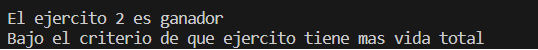
\includegraphics[width=0.5\textwidth,keepaspectratio]{img/captura6.png}
		%\includesvg{img/automata.svg}
		%\label{img:mot2}
		%\caption{Product backlog.}
	\end{figure}
	
	\begin{itemize}	
		\item Ya que el ejército 2 tiene 15 de vida, mientras que el 1 tiene 7. 
	\end{itemize}
	
	\begin{figure}[H]
		\centering
	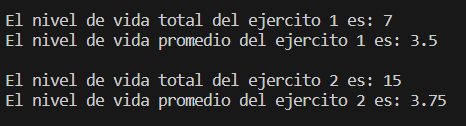
\includegraphics[width=0.5\textwidth,keepaspectratio]{img/captura7.png}
		%\includesvg{img/automata.svg}
		%\label{img:mot2}
		%\caption{Product backlog.}
	\end{figure}
	
	\section{\textcolor{red}{Rúbricas}}
	
	\subsection{\textcolor{red}{Entregable Informe}}
	\begin{table}[H]
		\caption{Tipo de Informe}
		\setlength{\tabcolsep}{0.5em} % for the horizontal padding
		{\renewcommand{\arraystretch}{1.5}% for the vertical padding
		\begin{tabular}{|p{3cm}|p{12cm}|}
			\hline
			\multicolumn{2}{|c|}{\textbf{\textcolor{red}{Informe}}}  \\
			\hline 
			\textbf{\textcolor{red}{Latex}} & \textcolor{blue}{El informe está en formato PDF desde Latex,  con un formato limpio (buena presentación) y facil de leer.}   \\ 
			\hline 
			
			
		\end{tabular}
	}
	\end{table}
	
	\clearpage
	
	\subsection{\textcolor{red}{Rúbrica para el contenido del Informe y demostración}}
	\begin{itemize}			
		\item El alumno debe marcar o dejar en blanco en celdas de la columna \textbf{Checklist} si cumplio con el ítem correspondiente.
		\item Si un alumno supera la fecha de entrega,  su calificación será sobre la nota mínima aprobada, siempre y cuando cumpla con todos lo items.
		\item El alumno debe autocalificarse en la columna \textbf{Estudiante} de acuerdo a la siguiente tabla:
	
		\begin{table}[ht]
			\caption{Niveles de desempeño}
			\begin{center}
			\begin{tabular}{ccccc}
    			\hline
    			 & \multicolumn{4}{c}{Nivel}\\
    			\cline{1-5}
    			\textbf{Puntos} & Insatisfactorio 25\%& En Proceso 50\% & Satisfactorio 75\% & Sobresaliente 100\%\\
    			\textbf{2.0}&0.5&1.0&1.5&2.0\\
    			\textbf{4.0}&1.0&2.0&3.0&4.0\\
    		\hline
			\end{tabular}
		\end{center}
	\end{table}	
	
	\end{itemize}
	
	\begin{table}[H]
		\caption{Rúbrica para contenido del Informe y demostración}
		\setlength{\tabcolsep}{0.5em} % for the horizontal padding
		{\renewcommand{\arraystretch}{1.5}% for the vertical padding
		%\begin{center}
		\begin{tabular}{|p{2.7cm}|p{7cm}|x{1.3cm}|p{1.2cm}|p{1.5cm}|p{1.1cm}|}
			\hline
    		\multicolumn{2}{|c|}{Contenido y demostración} & Puntos & Checklist & Estudiante & Profesor\\
			\hline
			\textbf{1. GitHub} & Hay enlace URL activo del directorio para el  laboratorio hacia su repositorio GitHub con código fuente terminado y fácil de revisar. &2 &X &2 & \\ 
			\hline
			\textbf{2. Commits} &  Hay capturas de pantalla de los commits más importantes con sus explicaciones detalladas. (El profesor puede preguntar para refrendar calificación). &4 &X &2 & \\ 
			\hline 
			\textbf{3. Código fuente} &  Hay porciones de código fuente importantes con numeración y explicaciones detalladas de sus funciones. &2 &X &2 & \\ 
			\hline 
			\textbf{4. Ejecución} & Se incluyen ejecuciones/pruebas del código fuente  explicadas gradualmente. &2 &X &2 & \\ 
			\hline			
			\textbf{5. Pregunta} & Se responde con completitud a la pregunta formulada en la tarea.  (El profesor puede preguntar para refrendar calificación).  &2 &X &2 & \\ 
			\hline	
			\textbf{6. Fechas} & Las fechas de modificación del código fuente estan dentro de los plazos de fecha de entrega establecidos. &2 &X &2 & \\ 
			\hline 
			\textbf{7. Ortografía} & El documento no muestra errores ortográficos. &2 &X &2 & \\ 
			\hline 
			\textbf{8. Madurez} & El Informe muestra de manera general una evolución de la madurez del código fuente,  explicaciones puntuales pero precisas y un acabado impecable.   (El profesor puede preguntar para refrendar calificación).  &4 &X &4 & \\ 
			\hline
			\multicolumn{2}{|c|}{\textbf{Total}} &20 & &18 & \\ 
			\hline
		\end{tabular}
		%\end{center}
		%\label{tab:multicol}
		}
	\end{table}
	
\clearpage

\section{Referencias}
	\begin{itemize}
		\item Fundamentos de la programación 2 - Tópicos de la programación Orientada a Objetos (Marco Aedo)
	\end{itemize}
	
%\clearpage
%\bibliographystyle{apalike}
%\bibliographystyle{IEEEtranN}
%\bibliography{bibliography}
			
\end{document}
